\documentclass{beamer}
\usepackage{fontspec}
\usepackage{xeCJK}
\setCJKmainfont{SimSun}  
\setCJKsansfont{SimHei} 
\usetheme{Madrid} % 使用 Madrid 主题
\usepackage{tikz}
\usepackage{graphicx}
\usepackage{ctex}
\usepackage{amsmath}
\usepackage{amssymb}
\usepackage{setspace}
\usepackage{float}
\usepackage{caption}
\usepackage{changepage}
\usepackage[ruled,linesnumbered,lined,boxed,commentsnumbered]{algorithm2e}
\usepackage{xcolor}
\usepackage[absolute,overlay]{textpos}
% 设置caption的格式
\captionsetup[figure]{labelformat=empty, labelsep=space, font=scriptsize, textfont=smaller}
% 隐藏导航键
\setbeamertemplate{navigation symbols}{}
% 定义颜色
\definecolor{deepblue}{RGB}{18, 52, 88}   
\definecolor{miblue}{RGB}{27, 78, 133}
\definecolor{lightblue}{RGB}{35, 104, 177} 
\definecolor{lightblue2}{RGB}{227, 236, 246} 
% 设置 Beamer 的颜色
\setbeamercolor{frametitle}{bg=lightblue,fg=white}
\setbeamercolor{title}{fg=white,bg=lightblue}
\setbeamercolor{section in head/foot}{bg=deepblue, fg=white}
%设置目录
\setbeamercolor{section in toc}{fg=lightblue}
\setbeamertemplate{section in toc}{%
	\leavevmode\leftskip=2em\large\heiti
	{\usebeamerfont*{section number projected}%
		\usebeamercolor[bg]{section number projected}%
		
\begin{tikzpicture}
			\node[rectangle, draw=none, inner sep=1pt, fill=lightblue2, minimum size=1.5em] (num) {\color{black}\inserttocsectionnumber};
	\end{tikzpicture}}%
	\hskip1em\inserttocsection\par}
\setbeamertemplate{subsection in toc}{
	\leavevmode
	\usebeamerfont*{subsection in toc}
	\hspace{4em}
	\makebox[1em][l]{\hfill}
	\inserttocsubsection\par
	\vspace{1ex}}
% 自定义页眉页脚
\setbeamerfont{section in head/foot}{size=\fontsize{7pt}{13pt}\selectfont}
\setbeamercolor{right foot}{bg=lightblue, fg=white}
\setbeamercolor{center foot}{bg=miblue, fg=white}
\setbeamercolor{left foot}{bg=deepblue, fg=white}
\setbeamertemplate{headline}{
	\leavevmode%
   \begin{beamercolorbox}[wd=.8\paperwidth,ht=2.5em,dp=1.25em,center,sep=0pt]{section in head/foot}
	\usebeamerfont{section in head/foot}\insertsectionnavigationhorizontal{.75\paperwidth}{\hfill}{\hfill}
   \end{beamercolorbox}%
\begin{beamercolorbox}[wd=.2\paperwidth,ht=2.5em]{subsection in head/foot}
	\hfill\raisebox{-0.335\height}{
\includegraphics[height=3.73em, keepaspectratio]{Jilin University.jpg}}
\end{beamercolorbox}%
}
\setbeamertemplate{footline}
{
	\leavevmode%
	\hbox{%
		\begin{beamercolorbox}[wd=.37\paperwidth,ht=2.5ex,dp=1ex,center]{left foot}
			\usebeamerfont{footline}\insertshortauthor(\insertshortinstitute) 
		\end{beamercolorbox}%
		\begin{beamercolorbox}[wd=.26\paperwidth,ht=2.5ex,dp=1ex,center]{center foot}
			\usebeamerfont{footline}June~~4,~2024 
		\end{beamercolorbox}%
		\begin{beamercolorbox}[wd=.37\paperwidth,ht=2.5ex,dp=1ex,center]{right foot}
			\usebeamerfont{footline}\insertshorttitle~~~~\insertframenumber/\inserttotalframenumber
	\end{beamercolorbox}}%
	\vskip0pt%
}


\title{方程求解的量子算法文献综述}
\author[李冠余]{
	{\fontsize{11pt}{13pt}\selectfont(本科生毕业论文答辩)}
	\vskip 15pt \hspace{-7pt}汇报人:李冠余
	\vskip 5pt 指导教师:某某~~教授}
\institute{吉林大学数学学院}
\date{}

\begin{document}
	\begin{spacing}{1.2}
	\setlength{\parindent}{1em}
	{\fontsize{8.5pt}{13pt}\selectfont
	\setbeamertemplate{institute}{}
	\begin{frame}%封面设置
		\vspace{-0.5cm}
		\titlepage
		\vfill
		\begin{textblock*}{5cm}(4.9cm,6.35cm)  
			
\includegraphics[width=1.8cm]{jd-xhh.jpg}  % 路径替换为院徽图片路径
		\end{textblock*}
		\vspace*{1cm}
		\centering{\small{June~~4,~2024}} 
	\end{frame}

    \section*{目录}
    	\begin{frame}
    		\frametitle{\secname}
    		\tableofcontents	
    	\end{frame}
    	\AtBeginSubsection[]{
    		\begin{frame}<handout:0>
    			\frametitle{目录}
    			\tableofcontents[currentsection,currentsubsection]
    		\end{frame}
    		\addtocounter{framenumber}{-1}  % 目录页不计算页码
    	}
  
    \section{研究现状}
    \subsection{问题背景}
    \begin{frame}
    \frametitle{维数灾难}
     在实际的应用当中,利用现有的数值方法,随着问题维度的不断增加,解决问题所需的计算复杂度也会呈指数级增长, 这种现象被称为”维数灾难”.例如:
     \vspace{5pt}
    		\begin{itemize}
    			\item \textbf{金融工程应用:}多资产期权定价需追踪多个相关资产,资产数量增加导致计算负担急剧增加.
    			\item \textbf{气候模型:}精确模拟大气和海洋流动需要在三维空间中解偏微分方程,全球气候系统模拟涉及成千上万的变量.
    			\item \textbf{机器学习与大数据:}高维数据集处理中,数据点稀疏和维数灾难导致模型易过拟合,影响泛化能力.
    		\end{itemize}
 \end{frame}

    \begin{frame}
    	\frametitle{量子优势}
    	量子具有叠加和纠缠的性质,理论上含有$N$个量子比特的系统可以同时表示$2^N$
    	个不同的状态, 但是传统的计算机如果是$N$个比特那也只能表示一个确定的数.\\
    	由于世界在本质上是量子力学的,并且任何物理过程以及定理(相对论除外)原则上都能很好的被量子计算机所模拟.所以,量子计算在原理上就是可以处理微分方程的.
 \end{frame}

\subsection{本文工作内容}
  \begin{frame}
  	  \frametitle{工作内容——电路模拟}
         使用qiskit设计了量子电路,对于基础的量子算法进行了模拟.
        \begin{figure}
        	\centering
        	\vspace{-0.2cm}
        	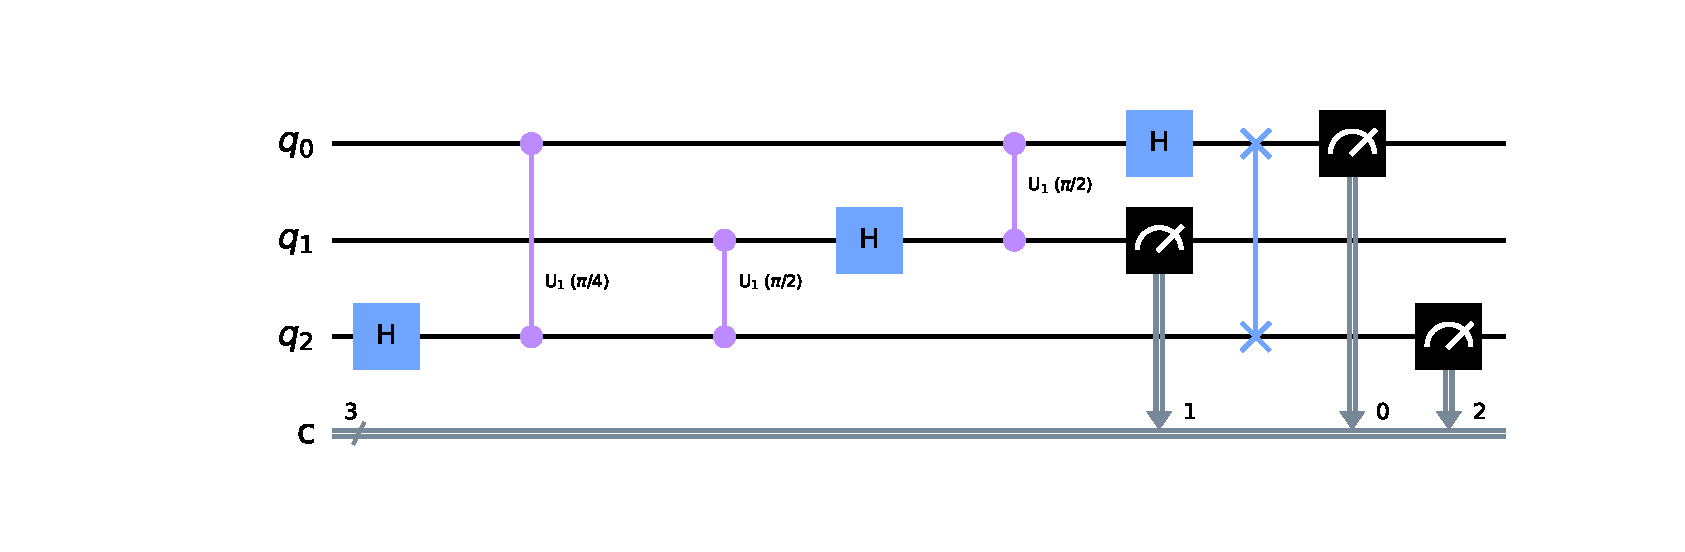
\includegraphics[width=0.65\textwidth]{qft.pdf}
        	\caption{图1~~量子傅立叶变换}
       
        	\begin{minipage}{0.45\textwidth}
        		\centering
        		\vspace{-0.3cm}
        		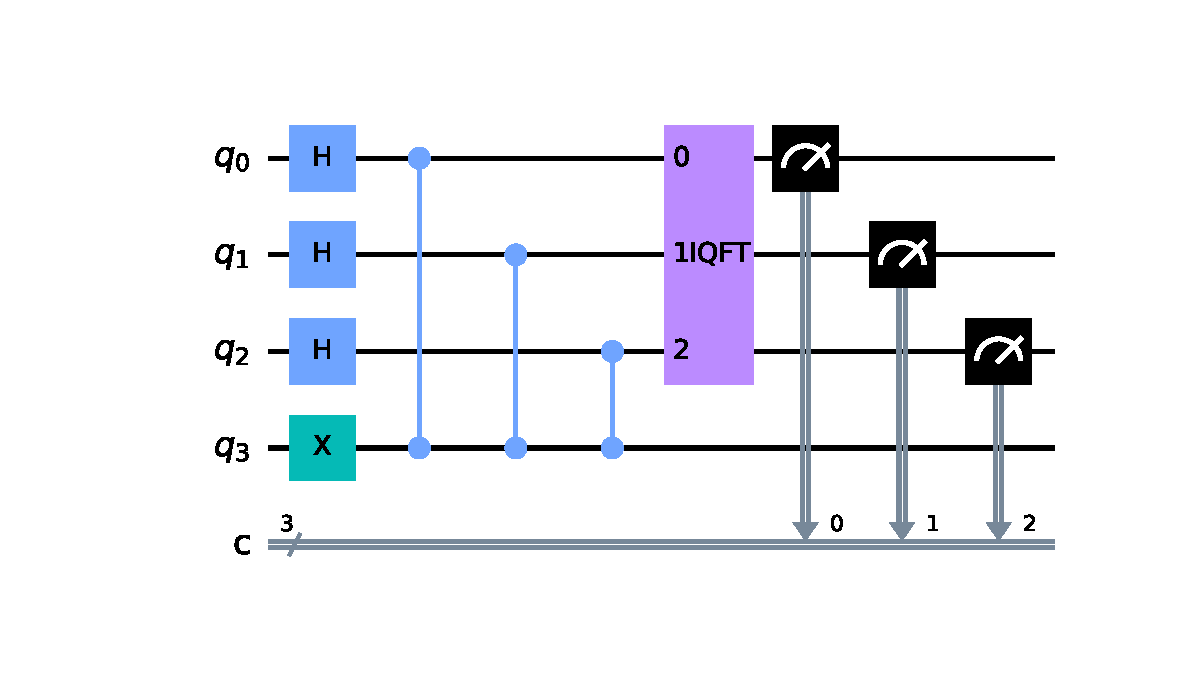
\includegraphics[width=\textwidth]{qpe.pdf}
        		\caption{图2~~量子相位估计}
        	\end{minipage}\hspace{0.02\textwidth}
        	\begin{minipage}{0.35\textwidth}
        		\centering
        		\vspace{-0.3cm}
        		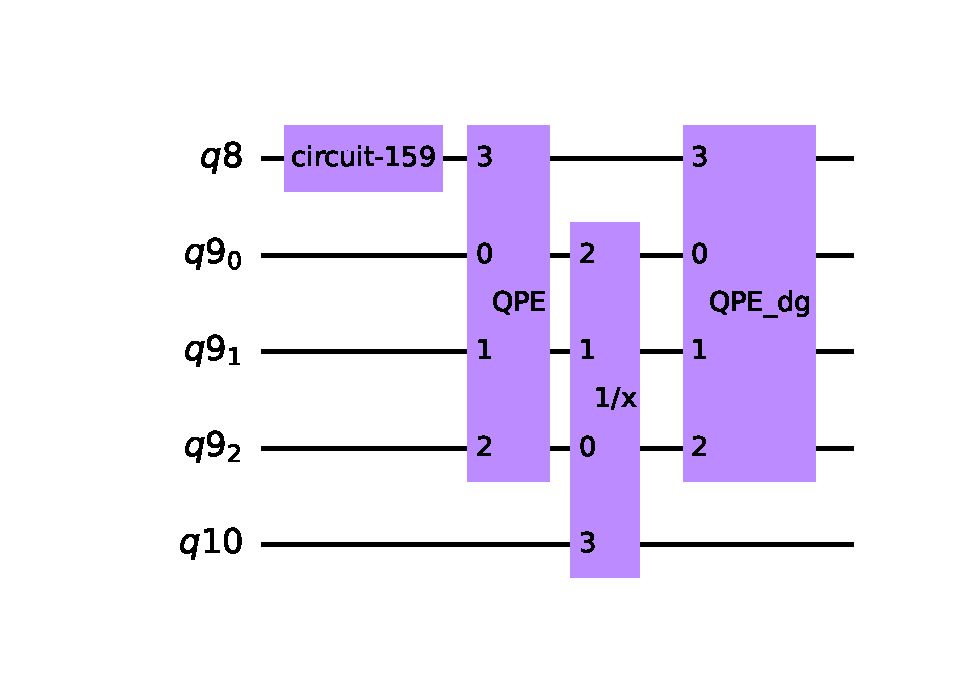
\includegraphics[width=\textwidth]{HHL.pdf}
        		\caption{图3~~HHL算法}
        	\end{minipage}
        \end{figure}
    \end{frame}

  \begin{frame}
  	\frametitle{工作内容——量子算法综述}
  	\begin{tabular}{p{0.5\textwidth} p{0.5\textwidth}}
  		\textbf{求解线性方程组:} &
  		\textbf{求解ODE:} \\ \hspace{-18pt}
  		\begin{minipage}[t]{0.5\textwidth}
  			\begin{itemize}
  				\item HHL 算法.
  				\item VQLS 以及各种变型.
  			\end{itemize}
  		\end{minipage} &\hspace{-18pt}
  		\begin{minipage}[t]{0.5\textwidth}
  			\begin{itemize}
  				\item 理论分析.
  				\item 离散化时间的方法.
  				\item 非离散化时间的方法(块编码).
  			\end{itemize}
  		\end{minipage} \\  	  
  	     \vspace{15pt} \\  
  		\textbf{求解线性PDE:} &
  		\textbf{求解非线性PDE:} \\ 
  		\hspace{-18pt}
  		\begin{minipage}[t]{0.5\textwidth}
  			\begin{itemize}
  				\item 离散化时间的方法.
  				\item 非离散化时间的方法(薛定谔化方法,虚时间演化法,块编码).
  			\end{itemize}
  		\end{minipage} &
  		\hspace{-18pt}
  		\begin{minipage}[t]{0.5\textwidth}
  			\begin{itemize}
  				\item 线性近似.
  				\item 直接表示.
  			\end{itemize}
  		\end{minipage}
  	\end{tabular}
  \end{frame}

    \section{算法综述}
    \subsection{求解线性方程组的量子算法}
    \begin{frame}
    	\frametitle{求解线性方程组的量子算法}
    	\textbf{HHL算法}
    	
    	考虑$A|x\rangle = |b\rangle ,$其中, $A$ 是厄米特矩阵($A \in \mathbb{C}^{N \times N}$ ).\\
    	故有谱分解~$A=\sum_{j=0}^{N-1}\lambda_j|u_j\rangle\langle u_j|, $则$A^{-1}=\sum_{j=0}^{N-1}\lambda_j^{-1}|u_j\rangle\langle u_j|. $  
    	然后把右侧按照 $A$ 的特征向量展开$|b\rangle = \sum_{j=0}^{N-1}b_j|u_j\rangle, $同时乘以$A^{-1}$, 得到$|x\rangle = A^{-1}|b\rangle = \sum_{j=0}^{N-1}\lambda_j^{-1}b_j|u_j\rangle.$
    	\vspace{20pt}
    	
        \textbf{变分量子求解器 (VQLS)}
        
        考虑 $M \in \mathbb{C}^{N \times N}$ 和向量 $|v_0\rangle$,想要得到规一化状态:
           $|v_M\rangle = \frac{M |v_0\rangle}{\|M |v_0\rangle\|}.$\\
        可以让$M$ 是非厄米特矩阵, $|v_M\rangle$ 是哈密顿量:
        $ H_M = I - \frac{M|v_0\rangle \langle v_0| M^\dagger}{\|M |v_0\rangle\|^2} $的基态,从而问题转化为寻找$H_M$的基态.
    \end{frame}

    \begin{frame}
         \frametitle{结论}
         
         HHL算法对于矩阵的条件数有很强的依赖,并且需要对量子比特进行精确细致的操作,所以实际使用中很容易受到噪声的影响导致结果出现错误.VQLS则更适合目前的有噪声的量子设备,其改进算法CQS也是其中唯一一个真正使用量子计算机进行测试并且解决实际意义的问题的算法,近期由于机器学习领域较为热门,该方法又可以使用专用量子退火机进行求解,因此潜力还是很大的.
    \end{frame}

     \subsection{求解常微分方程的量子算法}
     \begin{frame}
    	\frametitle{求解常微分方程的量子算法}
    	考虑常微分方程:
    	\begin{equation*}\label{eqn:ODE_general}
    		\left\{\begin{aligned}
    			&\frac{d}{dt} u(t)= Au(t) + b(t), \quad t \in [0,T], \\
    			&u(0) = u.
    		\end{aligned}\right.
    	\end{equation*}
    	其中 $u(t) \in \mathbb{C}^N$ 表示这个ODE的解, $A \in \mathbb{C}^{N\times N}$是系数矩阵,  $b(t) \in \mathbb{C}^N$ 是非齐次项. 
    	\vspace{10pt}
    	\begin{itemize}
    		\item 离散化时间的方法:~~把时间和空间全部离散化,然后使用HHL或者VQLS求解线性方程组.
    		\item 非离散化时间的方法:~~薛定谔化方法,块编码等.
    	\end{itemize}
    \end{frame}
    \begin{frame} 
    	\frametitle{结论}
       目前这些通过将时间和空间全部离散化之后再使用HHL算法以及其改进算法进行
     求解的量子算法, 对于ODE来说实际上量子优势还是比较微弱的,非离散化时间的方法中的块编码则对于系数矩阵$A$有较高的要求.总的来看,目前求解ODE的算法中,量子优势并不明显,再结合量子纠错目前的极高成本,该方向还是有很大的发展和进步空间的.
     \end{frame}
     
     \subsection{求解偏微分方程的量子算法}
     \begin{frame}
     	\frametitle{求解偏微分方程的量子算法}
     	\textbf{线性PDE}
     	
     	离散化时间的方法依然是把时间和空间全部离散化,然后使用HHL或者VQLS求解线性方程组.
     	
     	不离散化时间的方法和上面的ODE相同,通过快编码以及线性组合的玄正
     	技术包括虚时间演化法(只能做热方程),薛定谔化方法.

        \vspace{20pt}
        \textbf{非线性PDE}
        \begin{itemize}
        \item 线性近似: 通过做截断的方法将将非线性项线性化,尤其适用于非线性项是多项式的情况.
        \item 直接线性表示: 射线追踪,矩方法,水平集法.
         \end{itemize}              
     \end{frame}
    \begin{frame}
    	 \frametitle{结论}
		线性近似这种思路是将非线性项线性化,不过这种线性近似的办法会丢失部分非线性特征丢
		失,使得所描述的物理过程发生改变,并且只是在一段时间上有效果.而直接线性表示目前只适用于非常特定的方程,因此非线性PDE领域目前也还是很有进步空间的.
	\end{frame}
	
    \section{总结与展望}
      \begin{frame}
    \frametitle{总结与展望}
     \textbf{总结:}\\
     量子计算在求解线性方程组以及偏微分方程的方面展现出了巨大的潜力,相比于传统算法有着十分显著的优势.
     然而, 目前量子计算机在硬件上也面临着许多挑战, 如量子比特的稳定性和噪声影响等, 这在短
     时间内还是难以攻克的. 
     
    \vspace{20pt}
     \textbf{未来发展方向:}
    	\begin{itemize}
    		\item 针对特定问题开发量子模拟器(目前该领域硬件的发展会受到算法设计的影响).
    		\item 开发解决噪声和成本效益的量子纠错技术.
    		\item 结合传统方法,为当前量子计算机开发适用算法.
    		\item 在微分方程求解方面,更多的去研究无需时间离散化的算法.		
    	\end{itemize}
\end{frame}
}

{
	\setbeamertemplate{headline}{}
\begin{frame}
	\centering
	\Huge{感谢大家的聆听}
	
	\vspace{1cm}

	\normalsize{欢迎各位专家批评指正}
\end{frame}}
\end{spacing}
\end{document}
